\chapter{Background}
	\section{Introduction}
		\subsection{The Problem}
			Intellectual Property law is a term typically used to describe the areas of law which establish property protection over intangibles such as ideas, signs and information. This protection is in order to make the advancement of ideas profitable which therefore incentivises this act\cite{ip_edu_bently}.
			
			There is, therefore, a balance to be struck between limited exclusive rights and benefits to the public. While limiting exclusive rights may facilitate progress, benefiting the public, the overprotection of the exclusive property may restrict their access\cite{handbook_ip_hr_geiger}. One example of this is the expansion of copyright terms such as the contreversial Copyright Term Extension Act of 1998 which was heavily lobbied for by Disney just years before Mickey Mouse's copyright ran out\cite{mickey_mouse_grzelak}. The trend in extension of copyright terms, illustrated by Figure \ref{fig:ext_us_cop}, illustrates the appearance that the balance is tipping towards exclusivity rights. 

			\begin{figure}[h]
    			\centering
    			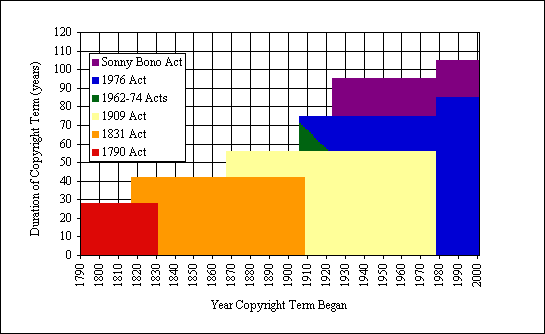
\includegraphics[width=0.5\linewidth]{resources/images/extention_of_us_copyright.png}
    			\caption{Expansion of U.S. copyright term lengths\cite{copyright_term_length_graph_bell}.}
    			\label{fig:ext_us_cop}
			\end{figure}
			
			
			This implementation of intellectual property law brings in the question of human rights of access to culture, education and other social and economic rights, but traditionally this has not been included in discussion of intellectual property law\cite{mapping_ip_hr_helfer}. However, recently scholarship and legislation has progrssively begun to incorporate each other's linguistics\cite{bileta_proposal_blakely}.
			
			
			Dr. Megan Rae Blakely of Lancaster University is looking for assistance in analysing journals and legal instruments for overlap in languages. In this analysis, I will map the dynamics of this change in legal and social perspective, to make evident moments of significant shifts in language. 
			
			
			Previously, analysis of the intersection between human rights and intellectual property law, such as Helfer's\cite{hr_ip_conflict_coexistence_helfer}, has been limited to more manual case-by-case methods. Supplying a more systematic method using natural language processing that can cope with large amounts of data would give concrete evidence of the relationship between human rights and intellectual proeprty. 
			\newpage
		\subsection{Aims and Objectives}
			In the early stages of the project, the following requirements for the project were established:
			\begin{itemize}
				\item A simple Graphical User Interface which allows for input of law journals and treaties PDF form.
				\item A visualisation of all inputted PDF documents with $x$-axis as time; $y$-axis as the intent of the document toward human rights to intellectual property; and $z$-axis as the measure of the extent to which the document suggests the protection of the creator/owner or the user.
				\item A code base written well enough for any future researcher to easily understand.
			\end{itemize}
			Over the course of the literature review, section \ref{sec:litrev}, I will review past literature in order to find the best methods to achieve each of these requirements.
		\subsection{Added Value}
			The originality of the project stems from its application of natural language processing methods in this domain, rather than the natural language processing methods used. The added value will be the unique way in which the findings are best illustrated for this application through the visualisation.
			
			The outcome of the project will help add value to its domain. As the first systematic, easily scalable technology in this domain, it will help illustrate how historical changes in technology have impacted the tone of intellectual law. Blakely points out that this, in turn, will allow legal professionals to consider how future technological changes will impact their work and adapt accordingly.
			\newpage
	\section{Literature Review} \label{sec:litrev}	
		\subsection{Natural Language Processing}
			The most common machine learning algorithm for 
			% 1. Support Vector Machines
			% 2. BOW v n-gram
			% 3. Word weighting
			% 4. Multi-labelled classifications
		\subsection{Graphical Representation}
			Abc
			% 1. 
		\subsection{User Interface}
			Abc
		\subsection{Documentation}
			Abc
	\section{Preliminary Investigation}
		\subsection{Preliminary Investigation}
			Abc
	\section{Project Plan}
		\subsection{Timeline}
			Abc
		\subsection{Evaluation}
			Abc